\def\bookfile{mother_of_hydrogen.pdf}
\def\booktitle{Mother of Hydrogen}

% Paper weight used
\input{papers}
\def\bookpaper{\lxxxgsm}


\newcounter{bookpagecount}
\setcounter{bookpagecount}{\XeTeXpdfpagecount"\bookfile"}
\RequirePackage{calc} % This line must be after the previous to avoid an error
\newlength{\outsidepaperwidth} % no. of pages ÷ 2 × width per sheet
\setlength{\outsidepaperwidth}{\bookpaper * \value{bookpagecount} / \real{2.0}}

\newlength{\outsidespinewidth} % paper thickness + 5mm
\setlength{\outsidespinewidth}{\outsidepaperwidth + 5mm}
\makeatletter
\setbox\z@=\hbox{\XeTeXpdffile"\bookfile"\relax}
\newlength{\outsidecoverwidth} % paper width + 8mm
\setlength{\outsidecoverwidth}{\the\wd\z@ + 8mm}
\newlength{\outsidecoverheight} % coverheight: paper height
\setlength{\outsidecoverheight}{\the\ht\z@ + 1mm}
\makeatother
% flapwidth: 60mm+3mm each side
\documentclass[12pt,coverwidth=\the\outsidecoverwidth,coverheight=\the\outsidecoverheight,spinewidth=\the\outsidespinewidth,marklength=0mm,bleedwidth=5mm,flapwidth=63mm]{bookcover}

\usepackage{contour}
\usepackage{moh}

% N.B. All text and images should be 6mm away from all edges
\begin{document}
\begin{bookcover}
    \bookcovercomponent{normal}{bg whole}{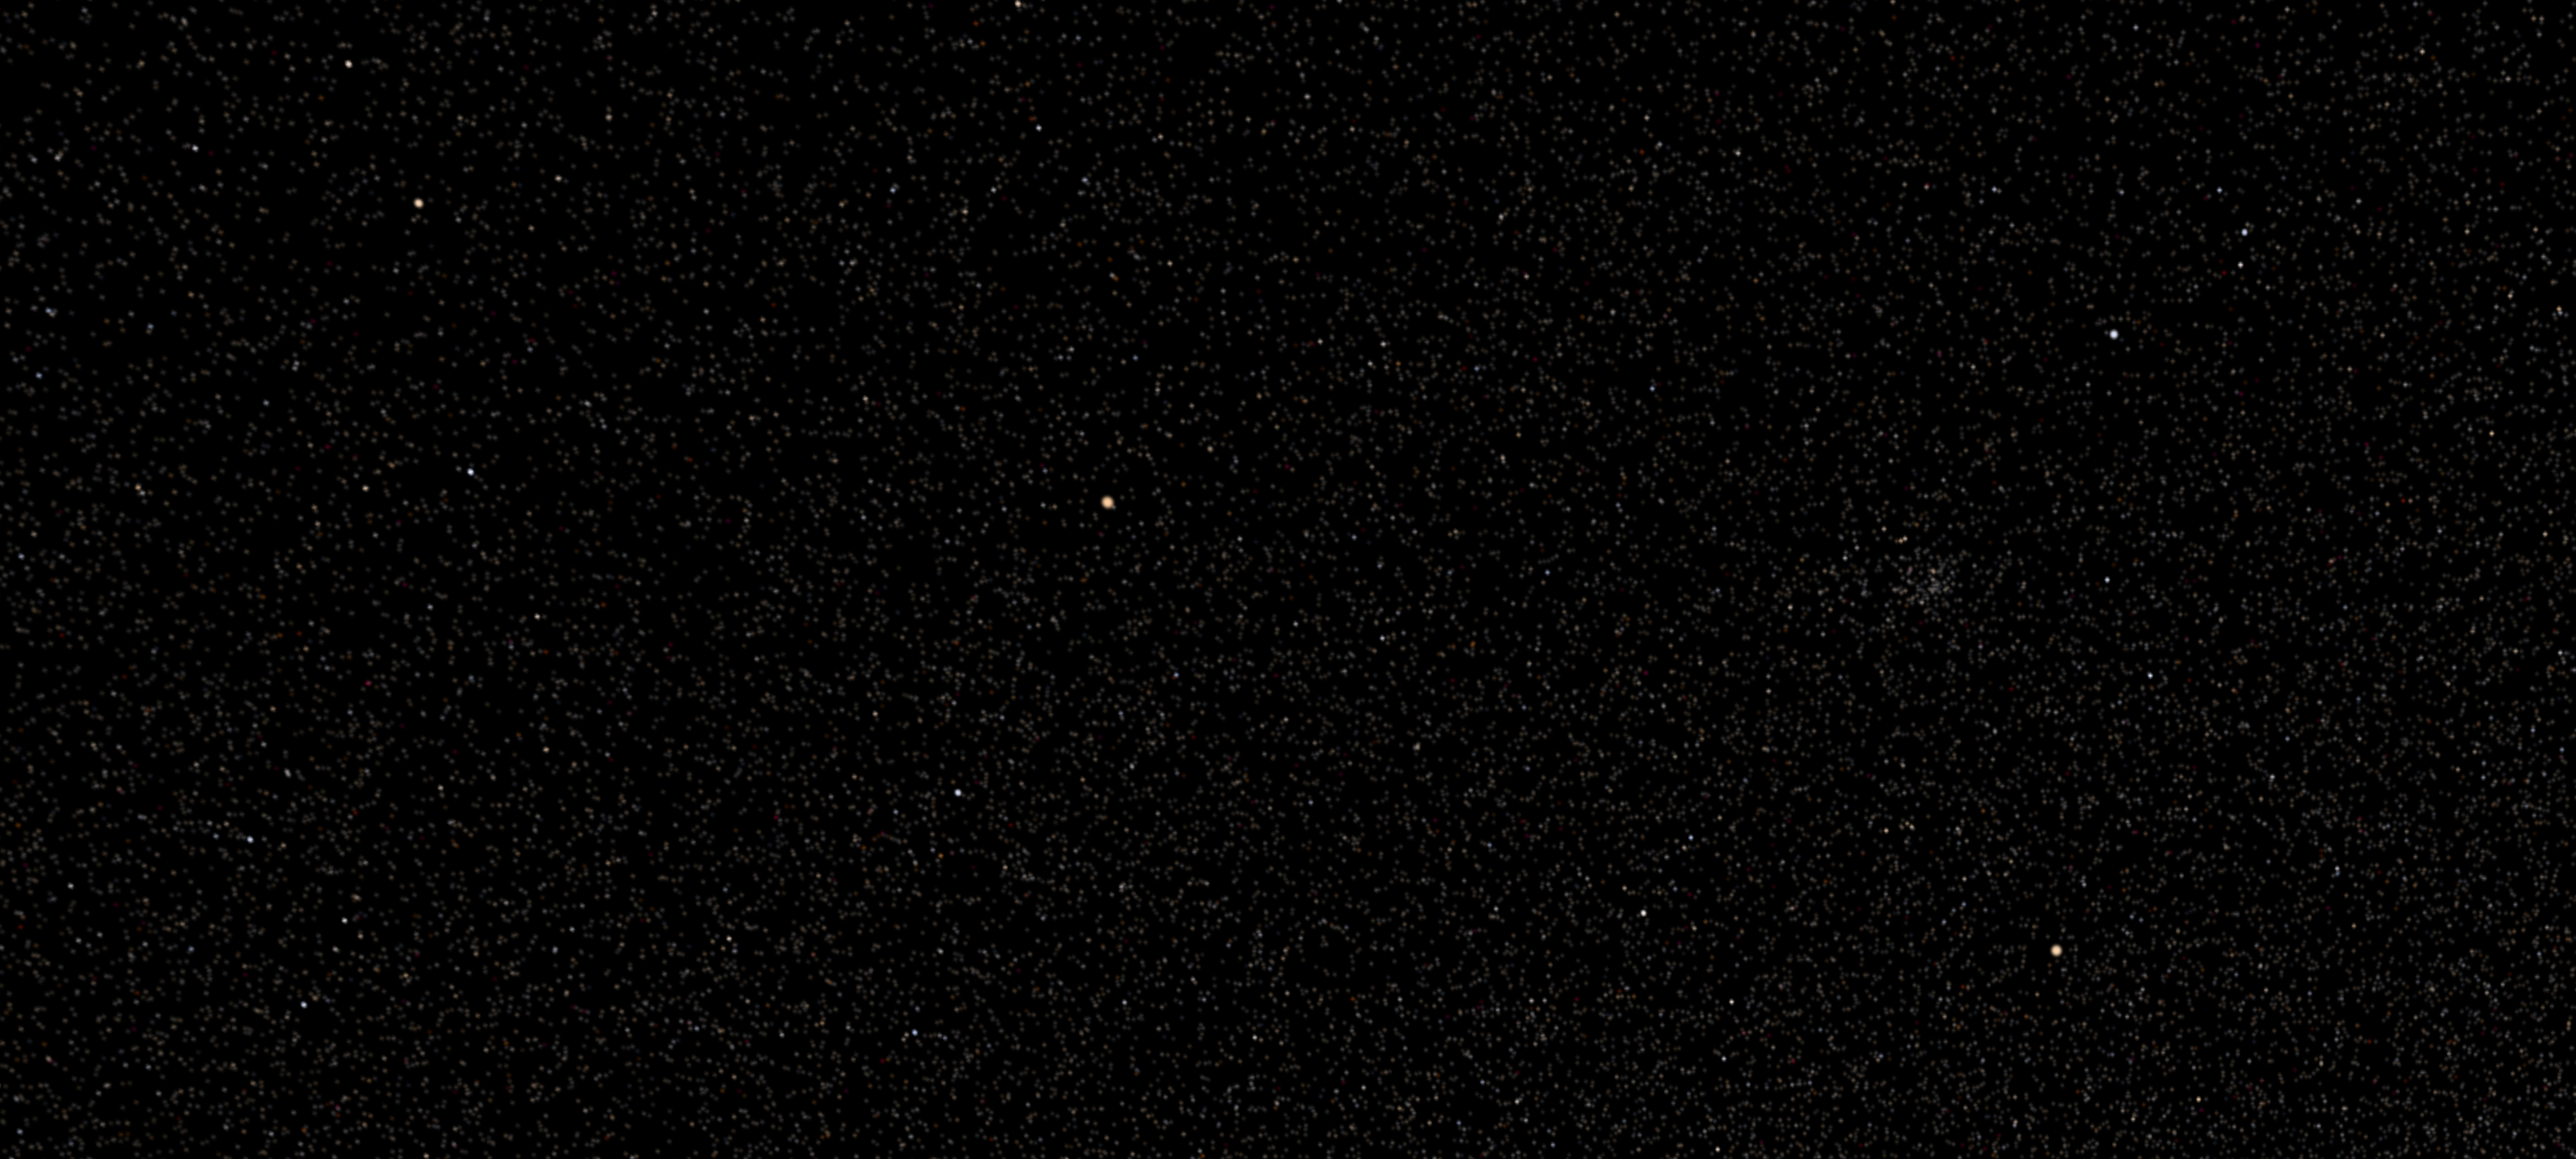
\includegraphics[width=550mm]{background.jpg}} % TODO: Why not 520mm, which is correct for aspect ratio?

  %\bookcovercomponent{normal}{front}{\color{white}\begin{center}\vspace{2cm}\bf{\Huge Mother of Hydrogen}\\[2cm]{\LARGE The Future We Deserve}\\[10cm]{\LARGE A Novel}\\[2cm]{\Huge Vinay Gupta}\\[2cm]{\Large Hexayurt Press}\end{center}}
  \bookcovercomponent{picture}{front}{Cover-transparent.png}

  \bookcovercomponent{center}{spine}{%
    \color{white}\LARGE\rotatebox[origin=c]{90}{\contour[120]{black}{\booktitle}}}

  \bookcovercomponent{normal}{back}{%
    \centering%
    \vspace{20mm}%
    \parbox{110mm}{\color{white}\Large\raggedright
      In the second half of the twenty-first century, a resurgent America dominates the world with its global humanitarian–military mission. Fifteen-year-old Harry Vine is about to start his mandatory national service. His father Gregory has reservations despite a career spent as a drone-jockey, and his uncle Peter, a hippie drop-out, is determined to prevent his joining the new brainwashed generation.

      Meanwhile in space, where all the really interesting tech is quarantined, an infant AI has become convinced it is the only conscious being in the known universe…
    }}


  \bookcovercomponent{normal}{front flap}{%
    \centering%
    \vspace{20mm}%
    \parbox{40mm}{\color{white}\raggedright\small
      In a world where the extremes of poverty and disease have been all but eliminated, what price a human soul? \emph{Mother of Hydrogen} shows us a future in which a state that’s not exactly totalitarian has given much of the planet a life that’s entirely bearable, and asks: how much is freedom really worth paying for? When there was no Faustian bargain to create a utopia, just a general agreement that a safer, more comfortable existence is worth paying for, how much compromise is too much?

      \bigskip Disaster relief specialist and unflinching futurist Vinay Gupta offers us a future sketched in shades of gray, and offers us an uncomfortable choice: black or white?}}

  \bookcovercomponent{normal}{back flap}{
    \centering%
    \vspace{20mm}%
    \parbox{40mm}{\color{white}\small\raggedright
      
\includegraphics[scale=0.1]{vinay.jpg}

      \bigskip Vinay Gupta is one of the world’s leading thinkers on infrastructure theory, state failure solutions, and managing global system risks including poverty/\allowbreak development and the environmental crisis.

      \bigskip He is trying to keep \emph{you} alive.
    }}
\end{bookcover}
\end{document}

% Local Variables:
% ispell-local-dictionary: "american"
% End:
